
\chapter{Interactive Tracking User Manual}
\label{chap:usermanint}

\section{Introduction}

This document aims to explain the new \emph{Interactive Tracking} feature developed during this thesis from the end-user's point of view. It will detail the steps required to use all new functions and to be able to recover a record using the new features.

As a prerequisite, the user must already be familiar with the existing PRISM and/or RENE programs to restore recordings acquired with IRENE. This document is focused on the version as integrated in PRISM. Almost all explanations in this document also apply to the RENE version. The differences are explained in \autoref{sec:inttrackrene}.

\section{General description}

\subsection{User interface overview}

In the application user interface, the main difference is the addition of a new panel on the right side, where the detailed record view also stands (see \autoref{fig:intpanel}). It is accessible by clicking on the \emph{Interactive Tracking} tab. The detailed view as already existing remains unchanged, and one can switch between the two views at any time. A new tracking option has also been added in the list of tracking methods.

\begin{figure}[!ht]
\centering
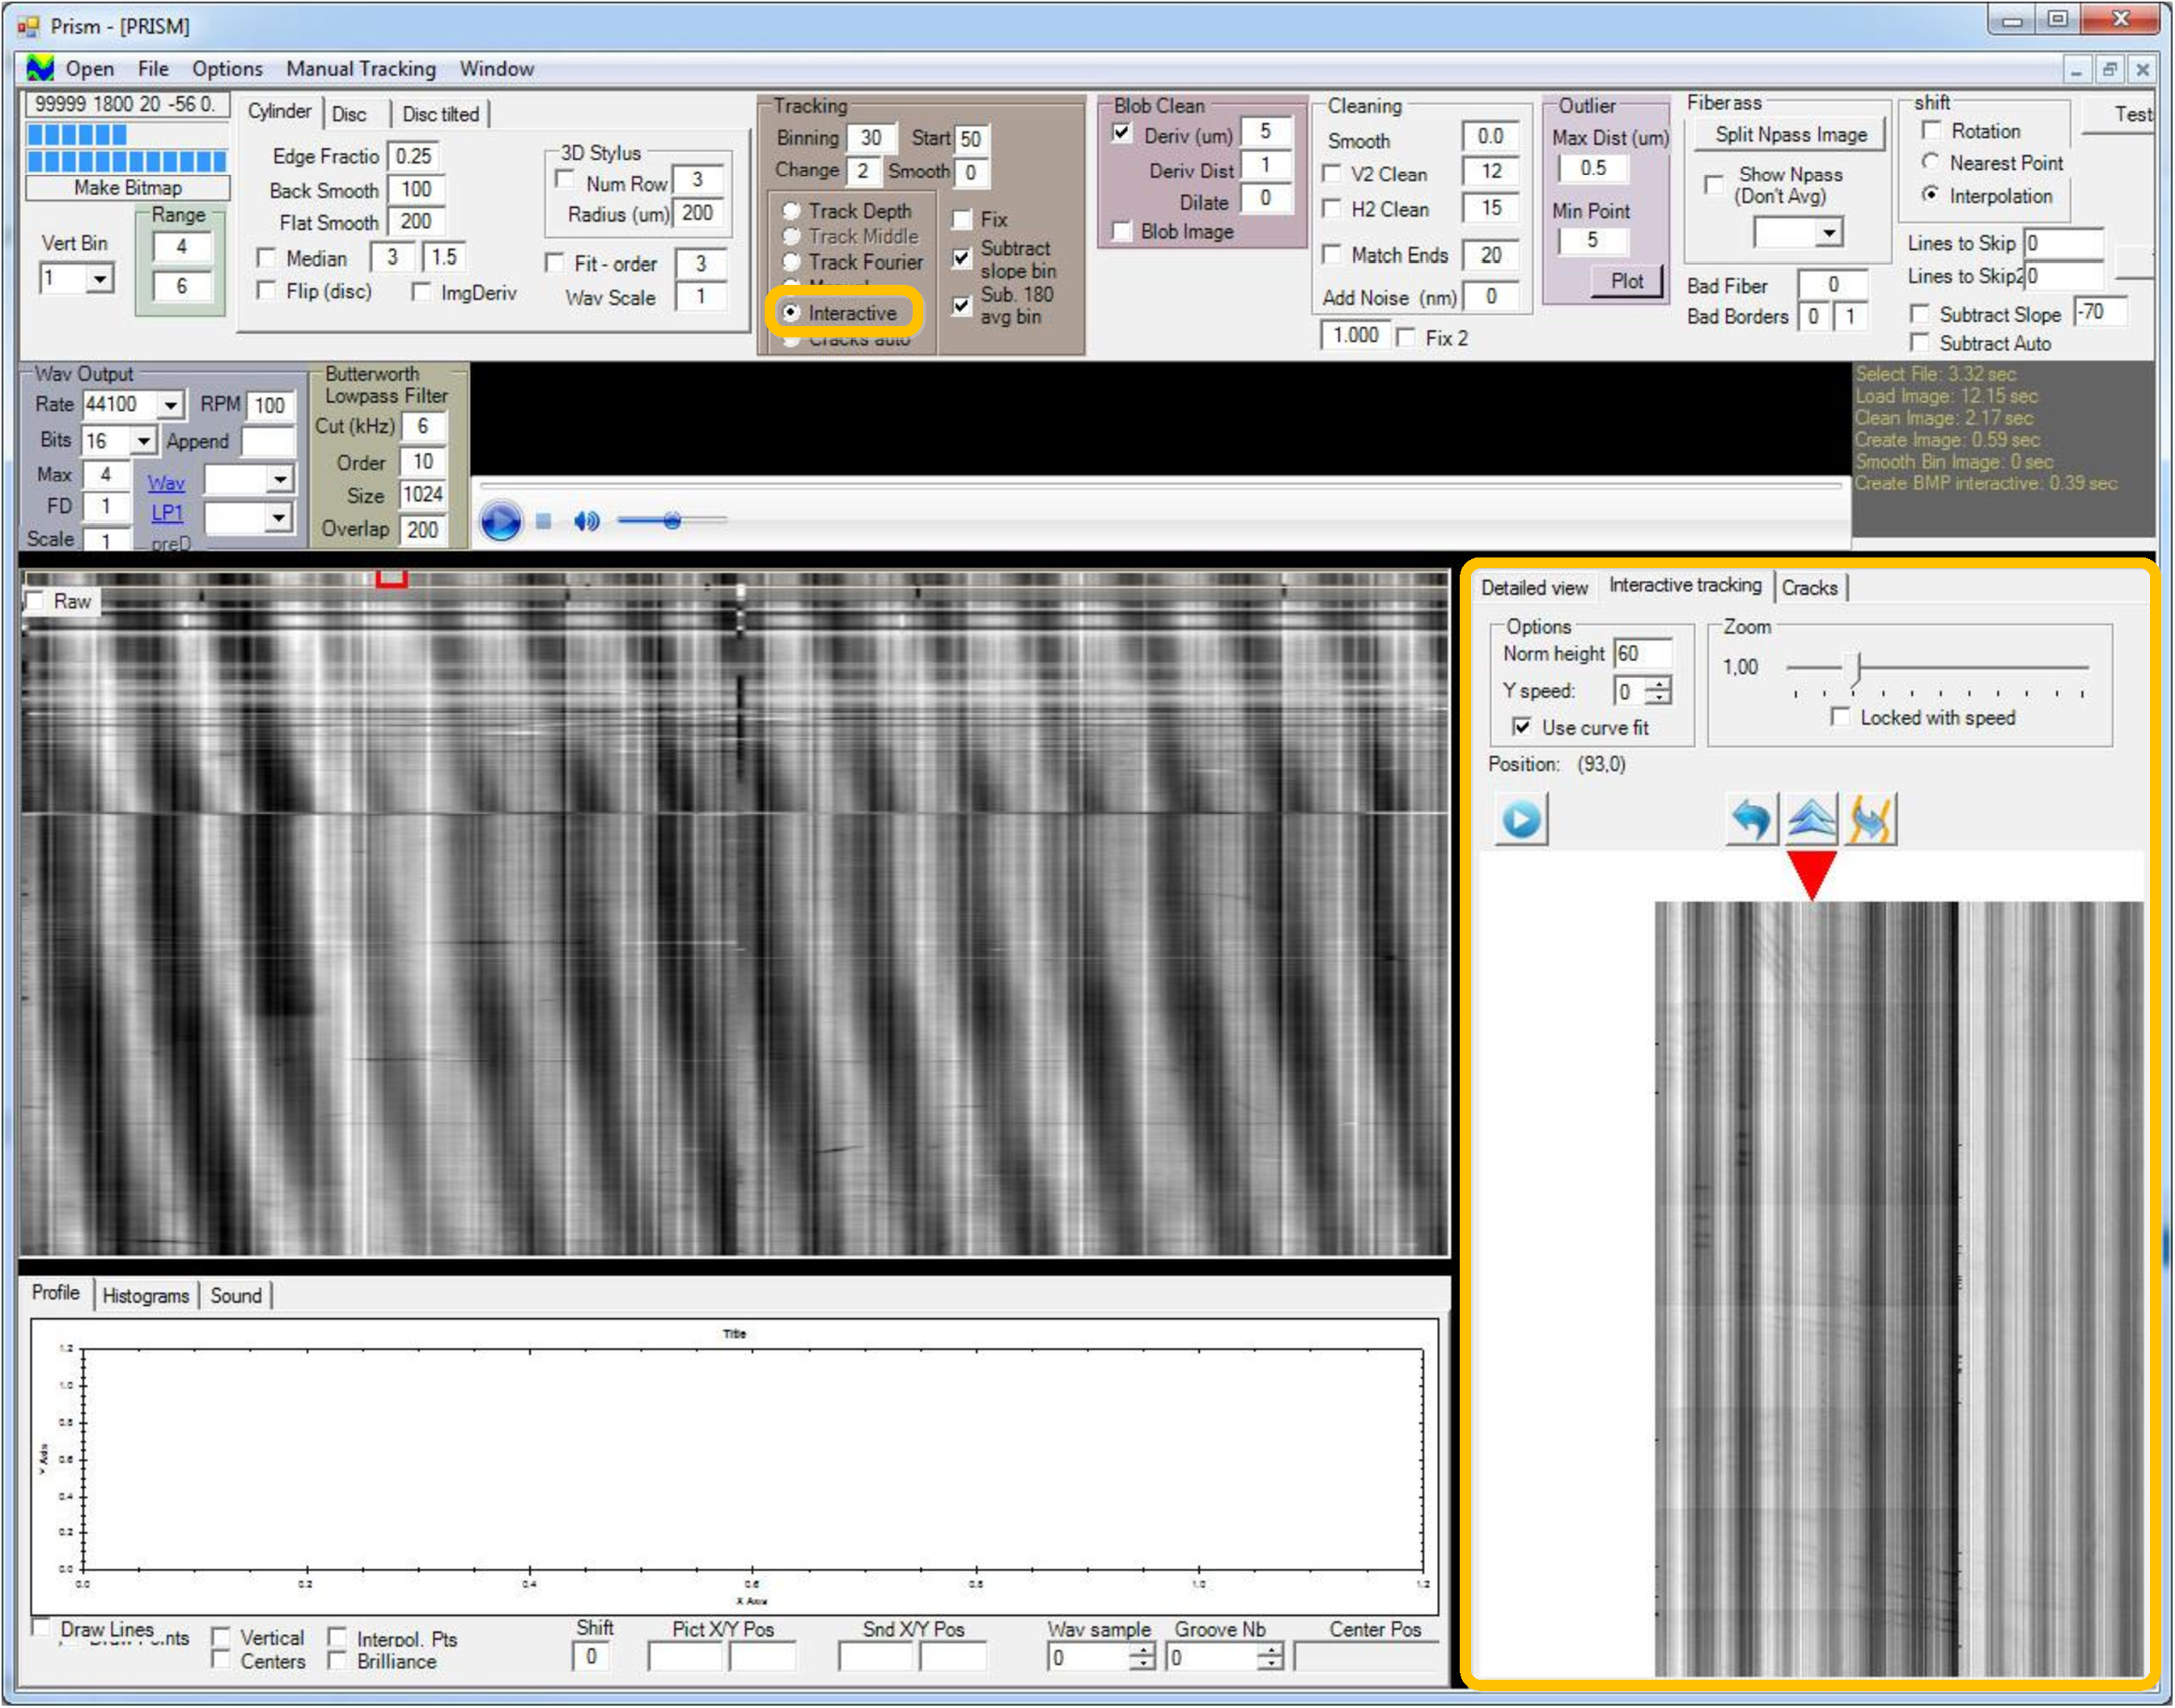
\includegraphics[width=0.9\textwidth]{images/int-right-panel}
\caption[Location of the interactive panel in PRISM.]
{Location of the interactive panel as well as the new tracking option highlighted in orange, as viewed in PRISM.}
\label{fig:intpanel}
\end{figure}

Almost all the new features are located on this panel. The upper part contains the controls and some information about the record being tracked. The remaining space is used to draw the record while tracking. When no record is loaded, this part is blank except for a red arrow.

A description of this panel can be seen in \autoref{fig:intguicontrols}. Specific controls are also detailed in \autoref{tab:intguicontrols}.

\begin{figure}[!ht]
\centering
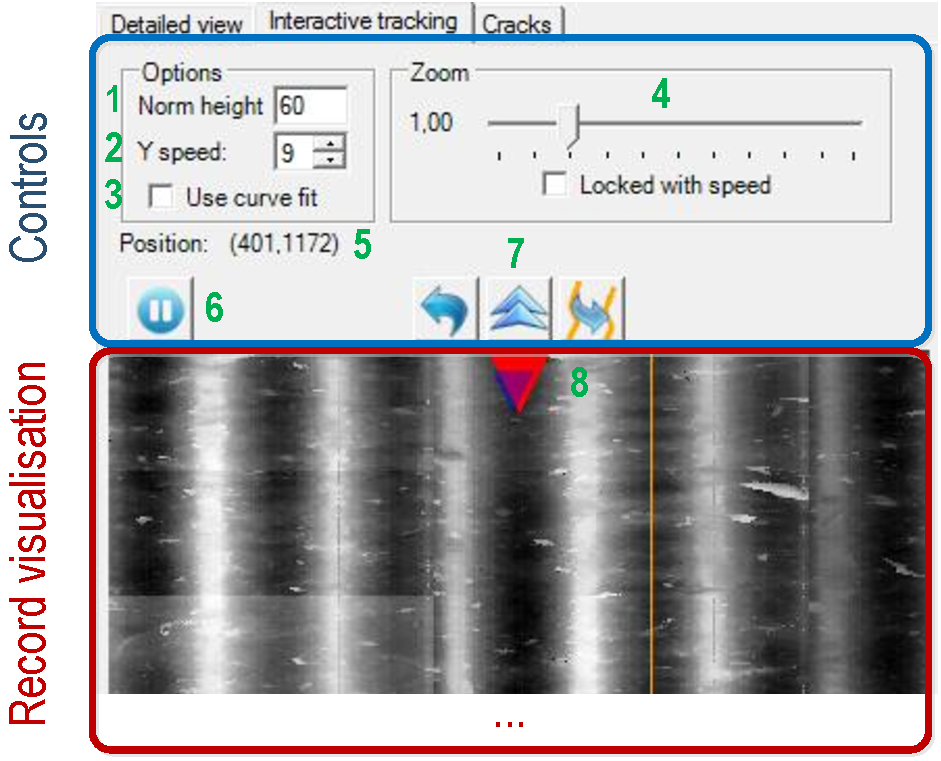
\includegraphics[width=0.6\textwidth]{images/int-track-controls}
\caption{Visualization of the controls in the interactive panel.}
\label{fig:intguicontrols}
\end{figure}

\begin{table}[h!]
\begin{center}
\tabulinesep=3pt
\begin{tabu} to 0.7\textwidth {| c | X[m] |} %{>{\bfseries}lX}
    \everyrow{\hline}
    \hline
    \rowfont[c] \bfseries
        No. & Description \\
        1 & Text box to change the height for bitmap contrast normalization (see \autoref{sec:contrastnorm}) \\
        2 & Tracking speed selector \\
        3 & Use curve fitting to make tracked position more smooth accurate \\
        4 & Zoom control \\
        5 & Indication of the current position pointed by the red arrow \\
        6 & Start/Stop tracking button \\
        7 & Tracking controls (see below) \\
        8 & Arrows indicating the currently tracked position \\
\end{tabu}
\end{center}
\caption{Explanation of the different objects in the interactive panel.}
\label{tab:intguicontrols}
\end{table}

\subsection{Description of controls}

The upper part enables to control different parameters for the tracking. The first one, \emph{Norm. height} may remain unchanged most of time. Its behavior is detailed in \autoref{sec:contrastnorm}. The \emph{Y speed} is for setting the speed while tracking a record. One can directly set the value or increment it. While tracking the record, it is also possible to increment and decrement the speed using the mouse wheel, without stopping the movement.

The option \emph{Use curve fit} enables to improve the tracking by adapting the center of the groove using parabola fitting. If unchecked, the smallest value in the neighborhood is defined as the real center.

To change the zoom level, whether to see more details or an overview of the scan, one can slide the \emph{Zoom} control. If the check box \emph{Locked with speed} is enabled, the zoom is automatically adjusted according to the tracking speed. This may be useful when a specific part needs a more accurate tracking. Slowing down will then directly show more details by expanding the zoom.

By default, the tracking is not active. To actually follow the groove, the \emph{Start/Stop} button must firstly be pressed. The tracking can be stopped at any time, e.g. to look over other parts and continue later.

\section{Loading a new acquisition}

Before loading the acquisition, the first step is to select the proper option, \emph{Interactive Tracking}, in the list of tracking types. Then, it remains to select the needed usual options for loading and processing and open the acquisition file into PRISM.

Once the record has been loaded, if the interactive tracking was selected, the heightmap image is directly viewed on the interactive panel, with the arrow pointing at the top-left corner.

\subsection{Contrast normalization}
\label{sec:contrastnorm}

The only option that must be set before loading the disc is \emph{Norm. height}. In some cases, the absolute surface height varies a lot on big areas, making the structure of grooves negligible and almost invisible if the contrast was normalized from the entire range of values (for more information, see \autoref{sec:contrastadj}). The original detailed view in PRISM is not directly concerned by this issue, as the contrast is readjusted each time the user selects a new area.

However, recomputing it would be too slow to draw the record interactively. Therefore, the normalization is performed in smaller area. The width corresponds to the width of a pass and the height may be controlled with this option. However, a value of 60 should be adequate in most situations.

\section{Tracking interactively}

This section details all options available to the user to help manually tracking a record as quickly and correctly as possible.

\subsection{Piloting the tracking}

In the interactive panel, the drawn record can be seen as a draggable object. When the mouse is pressed, it is possible to shift it horizontally by moving the cursor. The red arrow represents the currently tracked position and remains fixed at the top-center. It should therefore point at the center of the groove. An example of starting position can be seen in \autoref{fig:intshift}.

\begin{figure}[!ht]
\centering
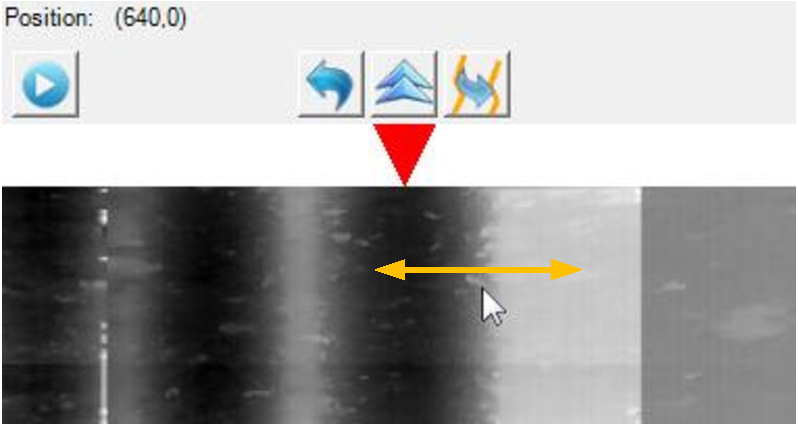
\includegraphics[width=0.7\textwidth]{images/int-mouse-shift}
\caption[Example of starting position.]
{Example of starting position. The record is dragged to the wanted position. The vertex of the arrow represents the position to be tracked. Here the tracking is not active, as the \emph{Start/Stop} button has not been pressed yet. In this specific case, the starting groove is located on the right (tracking from right to left).}
\label{fig:intshift}
\end{figure}

Once the groove as been selected, the tracking may start. To actually keep track of the position while moving, the \emph{Start/Stop} button must be pressed. Then, to start tracking, the most convenient way is to click on the record image and add speed using the mouse wheel. The image then starts scrolling down, representing the record being tracked.

The main goal is to keep the top of the arrow as close as possible to the groove center, ensuring a proper tracking. The speed can be adjusted at any time with the mouse wheel. The user can also release the click, change the speed on the control and click again on the record to continue tracking.

\subsection{On the binned image}

At any time, the current position can be viewed globally on the binned image as a little red square. This is very useful to locate the current position on the whole record. Another important feature is that it is also possible to click on the binned image to move to that position. If the tracking is enabled at this moment, this will also add a new tracking point. In fact, it will act the very same way as the former manual tracking. This is very useful when a specific area does not require a very precise analysis, enabling to track it very quickly.

The two views are always synchronized, each of them giving information at another level. The current path representing the part already tracked is also represented in orange. \autoref{fig:inttracksync2} represents an example of the part of a groove being tracked and visualized on both views.

\begin{figure}[!ht]
\centering
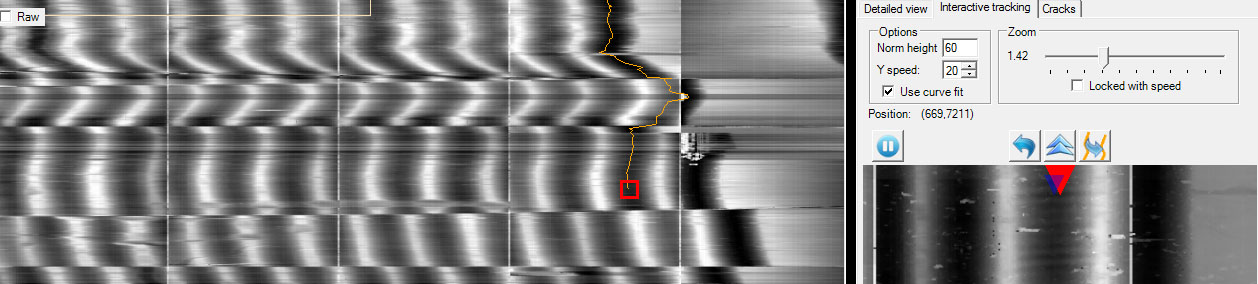
\includegraphics[width=1.0\textwidth]{images/int-track-sync-2}
\caption[A groove being tracked.]
{A groove being tracked. The two positions are synchronized and the path is drawn in orange.}
\label{fig:inttracksync2}
\end{figure}

\subsubsection{A magnifier tool}

When the cursor is moving over the binned image (without clicking on it) the portion viewed in the interactive panel is temporarily moved accordingly. This then acts as an interactive magnifier (adjustable with the zoom), which may be useful on a former analysis step or while tracking, e.g. to find the best matching when a crack appears.

\subsection{Starting a new revolution}

When an entire revolution has been performed, the final position is at the bottom of the mapped image. If the tracking is correct, the tracking may continue directly at the same horizontal position. The system is able to move back by setting a negative speed. However, to simplify this particular case (setting the position back to the top), a button has been added (upward pointing arrow). In reality, it does three things:

\begin{itemize}
\item Go back to the top (without changing horizontal position)
\item If the tracking is active, add a point at this position (representing the starting point of the new revolution)
\item Sets the speed to zero.
\end{itemize}

Resetting the speed is useful so that the position can be adjusted before continuing. The tracking can then start easily from this point. One can note that the tracking is drawn not only in the binned image, but also on the interactive panel, which gives a more detailed view of the result. It is also useful to compare the current track to the previous revolution. On the binned view, the link from the end to the start of the next revolution (conceptually the same position) is draw in red, as viewed in \autoref{fig:intnewrev}.

\begin{figure}[!ht]
\centering
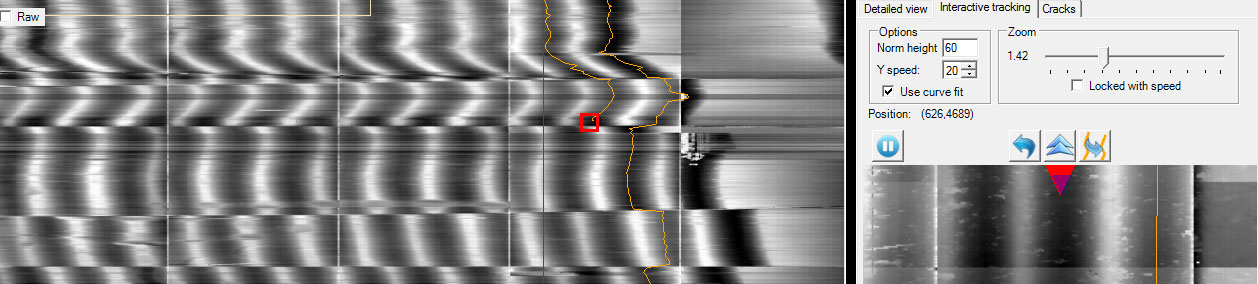
\includegraphics[width=1.0\textwidth]{images/int-new-rev}
\caption{Example when another revolution as started.}
\label{fig:intnewrev}
\end{figure}

\subsection{Letting the program do it}
\label{sec:assistracking}

Manual or interactive tracking are primarily useful with heavily damaged records that cannot be tracked with an automatic algorithm. However, though it is not directly possible to track e.g. over a crack, it could be possible to let the program find the way when on an area where no irregularity occurs.

This option is able to automatically track a section from the current position to a specified one, acting as an \emph{assisted} tracking. The user must simply press the \emph{Shift} key while clicking on the record. This way, it is not a straight line that is drawn but the real center is followed until the clicked position.

\subsection{Correcting an error}

Manually tracking a record is an error-prone process. It frequently happens that a particular point is wrong or that the a section of the track is wrong. An option to undo the last operation (leftwards arrow) has been added for this purpose. It reverses the new performed action and sets the position back to the previous one.

Usually, it directly removes the last tracked point. However, when the previous action added several points in one step, like with the assisted tracking or the copy pattern function (see \autoref{sec:assistracking} and \autoref{sec:copypattern}), it will directly remove the entire action, which is more convenient e.g. if the track was totally wrong in a too large section.

\subsection{Copying an existing pattern}
\label{sec:copypattern}

Another useful feature is the copy of a pattern that remains common between several revolution. It often happens that once the path has been found for a revolution (from top to bottom), the same pattern is repeated almost exactly in the same area.

To avoid doing the same job multiple times, the option (available through the last button on the GUI) automatically copies the pattern from the last revolution, starting at the current position and shifting it accordingly. An example of copied pattern is visualized in \autoref{fig:copypattern}.

\begin{figure}[!ht]
\centering
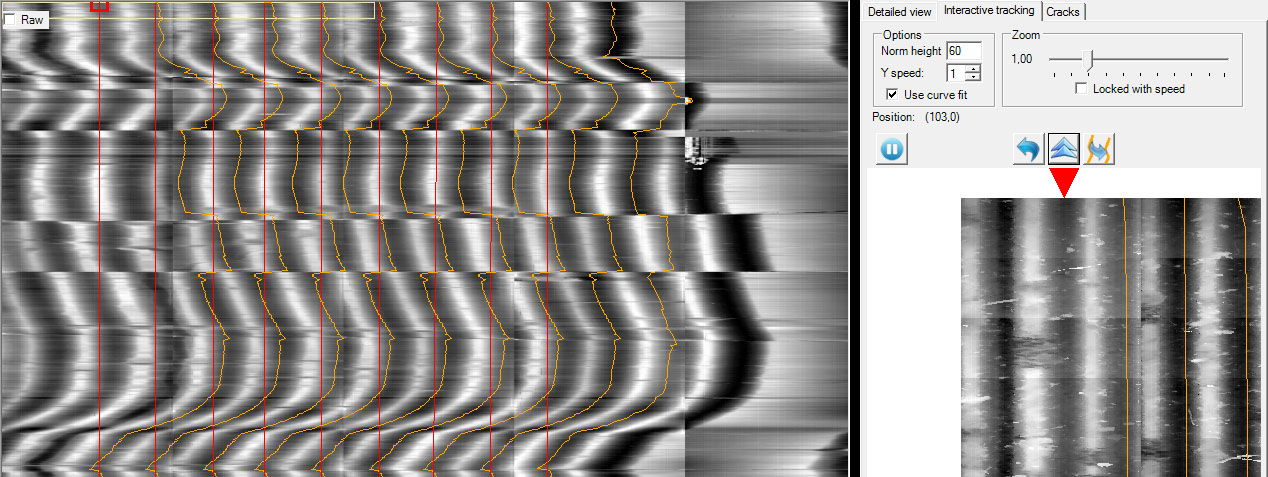
\includegraphics[width=1.0\textwidth]{images/int-copy-pattern}
\caption{Example of the same pattern copied for each revolutions.}
\label{fig:copypattern}
\end{figure}

For this feature to work properly, it is worth noting that the new revolution must have been previously started (i.e. the position has been put back to the top of the mapped image). The usual sequence is then (\texttt{Go to top}, \texttt{Copy}, \texttt{Go to top}, \texttt{copy}, \dots ). The horizontal shift may also be readjusted in between to precisely match the groove center. It may also be combined with the \emph{Undo} option.

\section{Starting record processing}

Once the tracking is completed, the remaining step is to launch the processing to finally get the audio file. In fact, this is done the same way as with the existing manual tracking. The \emph{Apply} action in the \emph{Manual Tracking} top menu will interpolate the track and launch the corresponding processing. The options can be set as usually regarding the record type (not detailed in this documentation).

\section{Other considerations}

\subsection{Saving and loading tracking}

This new way of tracking has been integrated in a way to minimize changes in the existing application. For the program, there is no difference between a record tracked with the old manual feature or with the new one. Thus, all existing options may also be used, as it is the case e.g. to apply the tracking and launch the processing.

Another useful feature already existing is the possibility to save the tracking to the hard drive, and load it back later on. The \emph{Load} and \emph{Save} options may be use as-is with the new implementation. The file is automatically saved in the record directory with a name postfixed by the starting range position. This enables to track several main parts of the record starting at different positions and at different times.

\subsection{Tracking direction}

Due to its way of operating, the interactive tracking can track only from \emph{top to bottom}, i.e. in one rotational direction. For records that have been recorded in the opposite direction, the acquired record must be flipped vertically at loading time, so that the sound will not be played backwards. This option already exists in both PRISM and RENE.

\section{Interactive tracking in RENE}
\label{sec:inttrackrene}

This section explains the difference in the implementation specifically for RENE. The first important thing is that the new tab is this time located on the left side of the user interface, as seen in \autoref{fig:intpanelrene}. The new tracking option has been added directly after the existing ones, in the \emph{Control} tab.

\begin{figure}[!ht]
\centering
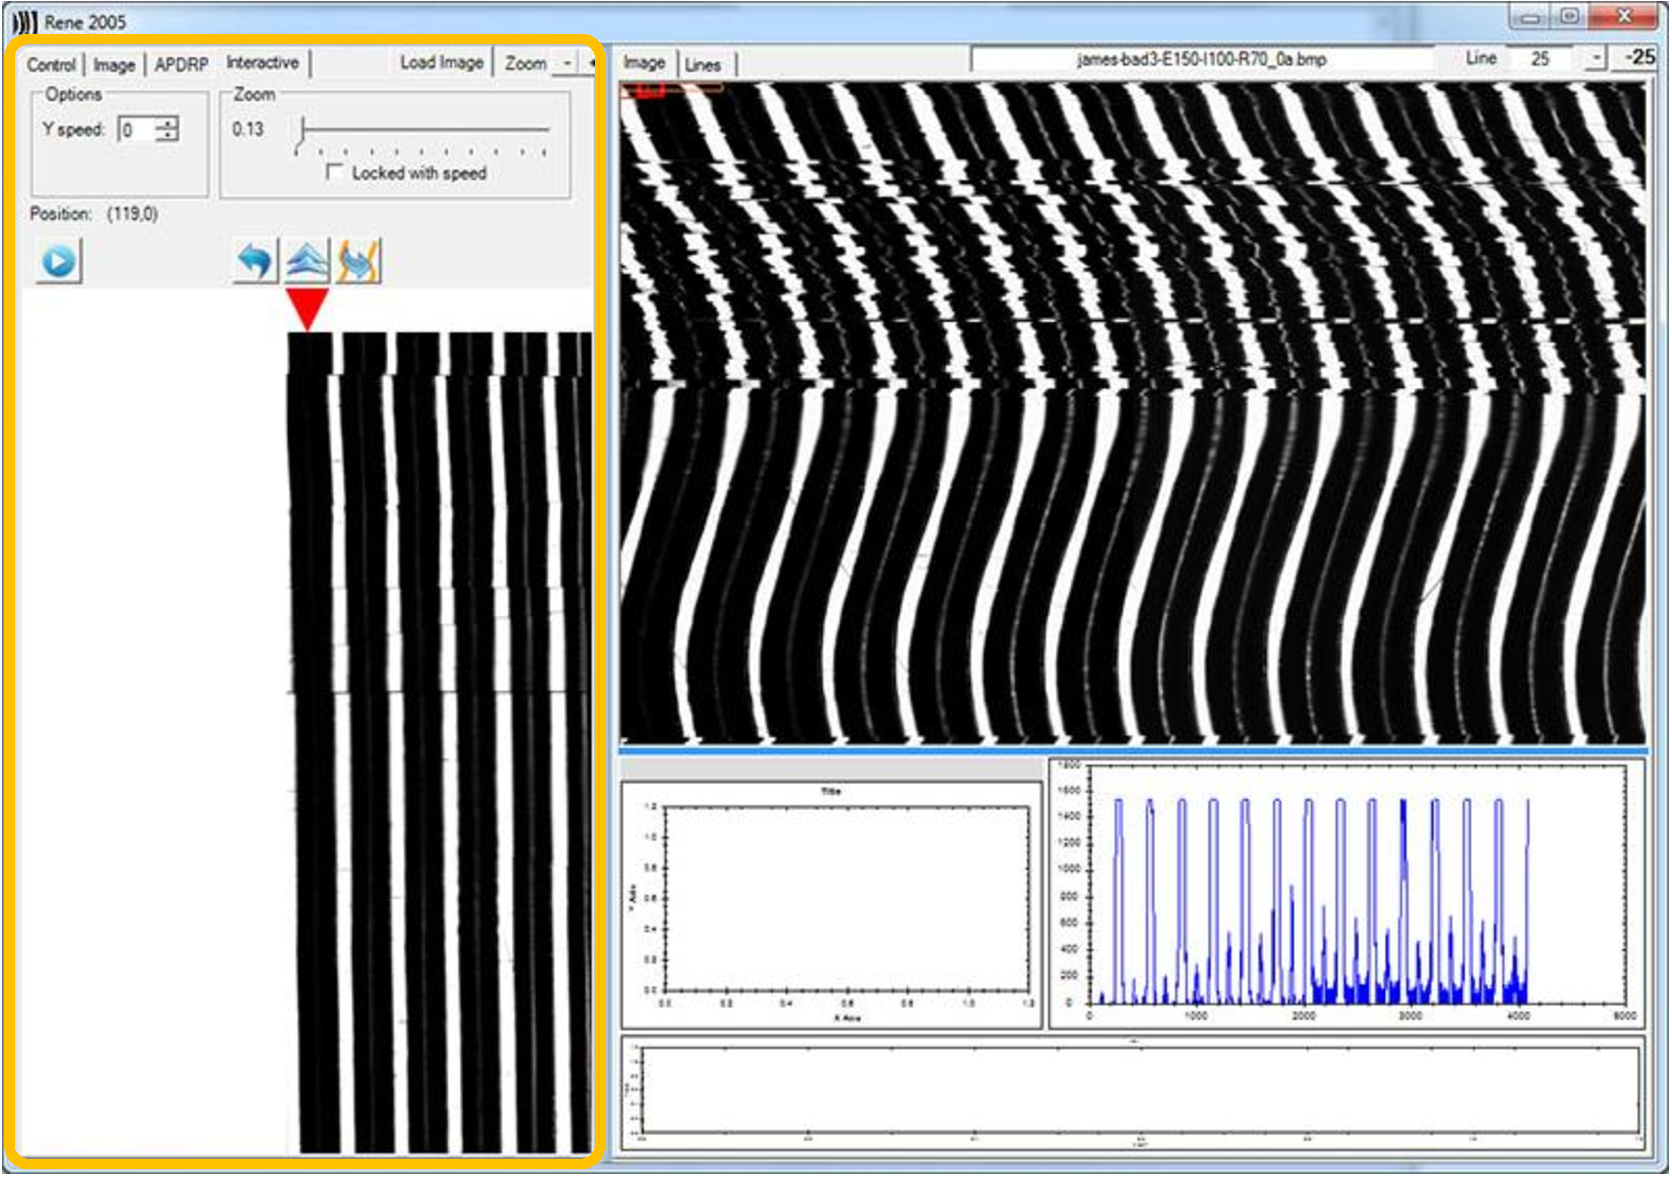
\includegraphics[width=0.9\textwidth]{images/int-right-panel-rene}
\caption[Location of the interactive panel in RENE.]
{Location of the interactive panel highlighted in orange, as viewed in RENE.}
\label{fig:intpanelrene}
\end{figure}

The other main change is the disappearance of the fit curve option. Indeed, with 2D acquisitions, this option is irrelevant. The tracking simply follows the brightest part representing the center of the groove.